%%%%%%%%%%%%%%%%%%%%%%%%%%%%%%%%%%%%%%%%%%%%%%%%%%%%%%%%%%%%%%%%%%%%%%%%%%%%%%%%%%%%%%%%%%%%%%%%%%%%%%%%%%%%%%%%%%%%%%%%%%%%%%%%%%%%%%%
%%| !!! TEMPLATE INSPIRED BY https://github.com/ocjojo/hska-latex-template                  !!! |%%
%%| !!! HsKa_old.jpg CAN BE FOUND HERE: https://de.wikipedia.org/wiki/Datei:Hska_logo.svg   !!! |%%
%%| !!! HsKa_new.png WAS CREATED BY USAGE OF IMAGERY FROM: https://www.h-ka.de/intern       !!! |%% 
%%%%%%%%%%%%%%%%%%%%%%%%%%%%%%%%%%%%%%%%%%%%%%%%%%%%%%%%%%%%%%%%%%%%%%%%%%%%%%%%%%%%%%%%%%%%%%%%%%%%%%%%%%%%%%%%%%%%%%%%%%%%%%%%%%%%%%%
%%| SET DOCUMENT PARAMTER HERE |%%
\documentclass[11pt]{article}

%%| INCLUDE PACKAGES HERE |%%
\usepackage[utf8]{inputenc}
\usepackage[paper=a4paper,left=25mm,right=25mm,top=25mm,bottom=25mm]{geometry}
\usepackage[english, ngerman]{babel}
\usepackage{graphicx}
\usepackage{amsmath}
\usepackage{amssymb}
\usepackage[autostyle=true,german=quotes]{csquotes}
\usepackage[backend=biber, style=ieee]{biblatex}
\usepackage{hyperref}
\usepackage{setspace}
\usepackage{microtype}
\usepackage{glossaries}
\usepackage{mdframed}
\usepackage{pgfplots}
\usepackage{algorithm}
\usepackage{algpseudocode}
\usepackage{amsmath}
\usepackage{array}
\usepackage{booktabs}
\usepackage[normalem]{ulem}
\usepackage{wrapfig}
\usepackage{listings}
\usepackage{xcolor}



%%| SET PACKAGE PARAMETERS HERE |%%
\hypersetup{                                                                        
    colorlinks,
    citecolor   = black,
    filecolor   = black,
    linkcolor   = black,
    urlcolor    = black,
    pdftitle    = {Machine Learning: Boosting-Algorithmen},                         
    pdfsubject  = {Seminararbeit},                                                  
    pdfauthor   = {David Erdös},                                                  
    pdfkeywords = {Machine Learning, Boosting, AdaBoost, Gradient Boosting} ,     
    pdfcreator  = {pdflatex},           
    pdfproducer = {LaTeX with hyperref}
}
\setstretch{1.25}                                                                  

%%| SET OTHER PARAMETERS HERE |%%
\addbibresource{Document/Bibliography/ref.bib}
\makeglossaries
\pgfplotsset{compat=1.17}
\renewcommand{\listalgorithmname}{Algorithmenverzeichnis}
% Definiere den Namen für \autoref für Algorithmen
\providecommand*{\algorithmname}{Algorithmus}
\providecommand*{\algorithmautorefname}{Algorithmus}
\useunder{\uline}{\ul}{}
\lstset{language=Python, 
        basicstyle=\ttfamily\small, 
        keywordstyle=\color{blue},
        commentstyle=\color{gray},
        stringstyle=\color{red},
        showstringspaces=false,
        breaklines=true}



%%%%%%%%%%%%%%%%%%%%%%%%%%%%%%%%%%%%%%%%%%%%%%%%%%%%%%%%%%%%%%%%%%%%%%%%%%%%%%%%%%%%%%%%%%%%%%%%%%%%%%%%%%%%%%%%%%%%%%%%%%%%%%%%%%%%%%%
%%| TITLE PAGE |%%
\begin{document}
\begin{titlepage}
    \begin{center}
        
\includegraphics[width=0.55\textwidth]{Images/Template/HsKa_new.png}\\[16ex]
        \huge{\textbf{-Machine Learning: Boosting-Algorithmen-}\\Seminararbeit}\\[8ex]
        \normalsize{}
        \begin{tabular}{lll}
            Student:            & \quad David Erdös                               & 67906 \\[2ex]
            Universität:        & \quad Hochschule Karlsruhe – Technik und Wirtschaft   &       \\[2ex]
            Studiengang:        & \quad Informatik Bachelor             &       \\[2ex]
            Semester:           & \quad Wintersemester 2023                             &       \\[2ex]
            Dozent:             & \quad Prof. Dr. Baier                       &       \\[2ex]
            Bearbeitet am:      & \quad 26. November 2023                             &       \\[2ex]
        \end{tabular}
    \end{center}
\end{titlepage}
\newpage

%%%%%%%%%%%%%%%%%%%%%%%%%%%%%%%%%%%%%%%%%%%%%%%%%%%%%%%%%%%%%%%%%%%%%%%%%%%%%%%%%%%%%%%%%%%%%%%%%%%%%%%%%%%%%%%%%%%%%%%%%%%%%%%%%%%%%%%
%%| TABLE OF CONTENTS |%%
\pagenumbering{gobble}    
\tableofcontents
\newpage
\pagenumbering{arabic}

%%%%%%%%%%%%%%%%%%%%%%%%%%%%%%%%%%%%%%%%%%%%%%%%%%%%%%%%%%%%%%%%%%%%%%%%%%%%%%%%%%%%%%%%%%%%%%%%%%%%%%%%%%%%%%%%%%%%%%%%%%%%%%%%%%%%%%%
%%| MAIN CONTENT |%%
\section{Einleitung}
Die voranschreitende Digitalisierung unserer Gesellschaft und die daraus folgende exponentielle Zunahme an Daten, hat Machine Learning als Schlüsselelement der modernen Datenanalyse ernannt. In den vielen Teilgebieten des maschinellen Lernens haben Boosting-Algorithmen einen besonderen Stellenwert. Besonders auf tabellarischen Datensätzen erbringen sie in vergleichsweise kurzer Trainingszeit in fast allen Benchmarks die besten Ergebnisse. Diese Seminararbeit konzentriert sich auf zwei Vertreter der Boosting-Familie: AdaBoost und Gradient Boosting Trees. Inhaltlich wird die Seminararbeit darauf abzielen, diese Algorithmen zu untersuchen und anhand eigener Beispiele zu erklären.

\subsection{Hintergrund und Motivation}
In der heutigen Zeit gibt es ständige Fortschritte im Bereich künstlicher Intelligenz. Nicht zuletzt mit der Veröffentlichung von Chat GPT ist die Benutzung von KIs zum Alltag geworden und wird auch von der breiten Masse genutzt. Als Student im Bereich der Informatik kann man es sich nicht mehr leisten, sich nicht mit den Themen der künstlichen Intelligenz zu beschäftigen. Die Fortschritte im Bereich der KI, wie sie Chat GPT demonstriert, haben sogar die lang angenommene Sicherheit des Berufs als Softwareentwickler beeinflusst. Zwar ist meine Einschätzung, dass KI-Systeme in naher Zukunft vorrangig als Werkzeuge benutzt werden und keine Berufsgruppen komplett ersetzen, doch selbst wenn ich falsch liege, ist davon auszugehen, dass diejenigen, die solche Tools entwickeln, als letzte ersetzt werden. Diese Überlegungen zur Zukunftssicherheit und die Erwartung, dass bahnbrechende Entwicklungen vor allem im KI-Bereich stattfinden werden, fördern mein Interesse schon seit längerem. Die Wahl des Themas dieser Seminararbeit spiegelt also mein Interesse an KI wieder und bietet eine gute Gelegenheit um sich mit Boosting-Algorithmen auseinanderzusetzten, was mir sicherlich in Zukunft zu gute kommen wird.

\subsection{AdaBoost und GradientBoosting: Ein Überblick}
AdaBoost war eins der ersten Beispiele für Boosting und wird als Stellvertreter für diese Kategorie gesehen. Die Grundidee in dem iterativen Prozess des Trainings die Gewichtung der Daten zu ändern, dass sie sich auf die Fehler fokussieren. Ähnlich dazu ist der GradientBoostingTrees, wobei dieser Algorithmus Entscheidungsbäume nutzt, welche auf dem Restfehler des Vorgängers trainiert werden.Beide Algorithmen nutzen das Prinzip der iterativen Verbesserung, allerdings auf unterschiedliche Weise, was ihre Anwendung in verschiedenen Kontexten und Aufgabentypen interessant macht.

\subsection{Zielsetzung und Struktur der Arbeit}
Diese Arbeit zielt darauf ab, die beiden genannten Algorithmen umfassend zu analysieren. Dabei wird ein Schwerpunkt auf die praktische Anwendung und die Veranschaulichung ihrer Funktionsweise durch eigene Beispiele gelegt. Der Aufbau der Arbeit ist wie folgt strukturiert: Zunächst wird ein grundlegendes Verständnis des Boosting-Konzepts geschaffen. Anschließend werden die Algorithmen AdaBoost und GradientBoosting detailliert beschrieben, wobei deren theoretische Grundlagen, Funktionsweisen im Vordergrund stehen, aber durch Beispiele veranschaulicht werden. Darauf aufbauend folgt eine direkte Gegenüberstellung beider Algorithmen, in der ihre Unterschiede, Vor- und Nachteile sowie optimale Einsatzgebiete diskutiert werden.



\cite[text]{Frochte2020}
\cite[text]{SchapireFreund2012}
\cite[text]{Geron2018}
\cite[text]{James2023}
\cite[text]{Hastie2009}
\section{Grundlagen des Machine Learning (3-4 Seiten)}
\subsection{Modern Approaches in Machine Learning}
Überblick über aktuelle Trends und Innovationen im Machine Learning
Vorstellung fortgeschrittener Techniken und Methoden
Diskussion über die Bedeutung von Deep Learning und künstlichen neuronalen Netzen
\subsection{Role of Boosting Algorithms in ML}
Einführung in Boosting-Algorithmen und ihre Relevanz
Spezifische Betrachtung von \gls{adaboost} und \gls{gradientboosting}
Vergleich von Boosting-Algorithmen mit anderen fortgeschrittenen Methoden
\subsection{Boosting Algorithms in Tabular Data Analysis}
Bedeutung von tabellenartigen Datensätzen in fortgeschrittenen ML-Anwendungen
Analyse, wie \gls{adaboost} und \gls{gradientboosting} bei tabellenartigen Daten effektiv sind
Fallstudien und Beispiele aus der Praxis, die den Einsatz dieser Algorithmen zeigen

Daten
Entscheidungsbäume
Traingsfehler
\section{Boosting}
Nach meiner eigenen Erfahrung als Student fällt oft auf, dass Gruppenarbeit nicht immer die erwarteten Vorteile bringt. Oft dominiert in Lerngruppen ein einzelner Student, der über fundiertes Wissen verfügt, die Diskussion und die Gruppenleistung spiegelt im Wesentlichen seine individuelle Leistung wider. 
\newline
In Fällen, wo alle Mitglieder einer Lerngruppe nur begrenztes Wissen zu einem Thema haben, kann die kollektive Leistung sogar hinter dem zurückbleiben, was man durch zufällige Antworten erwarten würde. Die Vorstellung, dass eine Gruppe von Individuen mit begrenztem Wissen gemeinsam Ergebnisse erzielen kann, die sowohl den Durchschnitt als auch jede individuelle Bestleistung übertreffen, widerspricht oft unserer Intuition. Selbst historische Weisheiten, wie sie in der Bibel gefunden werden, betonen die Risiken einer solchen Zusammenarbeit. Dort heißt es metaphorisch: ``Wenn aber ein Blinder den andern führt, so fallen sie beide in die Grube'' (Mt 23,16; Mt 23,24; Lk 6,39; Röm 2,19).
\newline
\newline
Doch im Bereich des maschinellen Lernens offenbart sich ein ganz anderes Szenario. Hier ermöglicht das Boosting-Verfahren, dass die Kombination von schwachen Modellen zu einem leistungsstarken Gesamtsystem führt. Dieser Ansatz, der die aggregierte Intelligenz mehrerer einfacher Modelle nutzt, um komplexe Probleme zu lösen, steht im starken Gegensatz zu den oft enttäuschenden Ergebnissen menschlicher Gruppenarbeit mit begrenztem Wissen \cite[S.~3]{SchapireFreund2012}.

\subsection{Was ist Boosting}
\begin{mdframed}
    \textbf{Boosting (ursprünglich Hypothesis Boosting)} bezeichnet eine beliebige Ensemble-Methode des Supervised Learning, bei der sich mehrere schwache Lerner durch Hintereinanderausführung (iterativ) zu einem starken Lerner kombinieren lassen. \textcite[S.~191]{Geron2018}. Das Boosting findet statt, indem die Fehler des Vorgängers stark höher gewichtet werden für die folgende Lerniteration als richtig erkannte Zuordnungen. So beschäftigt sich jede Lerninstanz primär mit der Ausmerzung der Fehler des Vorgängers.
    
Es gibt eine entfernte Verwandtschaft des Boostings zu der "Attention" in modernen Transformer-Architekturen wie GPT. Der meist verwendete Gradientenabstieg zur Fehlerminimierung in Boosting-Verfahren ähnelt wiederum den auch in Neuronalen Netzen verwendeten Gradientenabstiegsverfahren wie z.B. Backpropagation. Ein Unterschied sind jedoch meist wesentlich geringer benötigte Ressourcen und Lernzeiten als bei Deep Learning Modellen, wo sehr hohe Zahlen von Parametern nötig sind.

Zu einem bekannten anderen Verfahren des Ensemble Learning, den Random Forests besteht ein grundsätzlicher Unterschied: Random Forests sind **parallele** Lerninstanzen, deren Ergebnisse kombiniert werden, z.B. durch Mehrheitsentscheide, wohingegen Boosting Verfahren prinzipiell **sequentiell** ausgeführt werden, weil ja auf den Fehler des Vorgängers abgestellt wird. Andere Parallelisierungen sind natürlich möglich.\textcite[S.343]{Frochte202} Insbesondere können natürlich auch beim Boosting mehrere Klassifikatoren parallel betrachtet und kombiniert werden.

\subsection{Beispiel Wettererkennung}
\end{mdframed}

Die genannte Definition des Boosting lässt sich gut anhand des Beispiels der Wettererkennung veranschaulichen. Betrachten wir folgende einfache Regeln (Schwache Lerner) zur Beurteilung, ob es regnet:

\begin{table}[h]
    \centering
    \begin{tabular}{|l|l|}
    \hline
    \textbf{Schwache Lerner}      & \textbf{Grenzwert}   \\ \hline
    Nasser Boden               & Ja                  \\ \hline
    Wolken am Himmel           & Ja                  \\ \hline
    Hohe Luftfeuchtigkeit      & $>$ 80\%             \\ \hline
    Personen mit Regenschirm   & Ja                  \\ \hline
    Außentemperatur            & $>$ 0°C             \\ \hline
    \end{tabular}
    \caption{Individuelle Vorhersagen der Schwache Lerner}
    \label{tab:weak_learners}
\end{table}

Beispielsweise ist ein nasser Boden zwar eine Voraussetzung und ein guter erster Filter, allerdings könnte der Boden genauso gut durch einen Rasensprenger nass sein.
\newline
Die Temperatur ist hingegen ein relativ schlechtes Indiz für die Frage, ob es gerade regnet. Es unterscheidet aber den Fall Regen und Schnee und ist somit trotzdem essentiell für die Klassifikation.

\subsubsection{Erzeugung eines starken Lerners}
Der nächste Schritt ist es, die Aussagen der schwachen Lerner in ein nützliches Model zusammenzufassen, einen sog. `starken Lerner'. Im einfachsten Fall lässt man die schwachen Lerner mit gleicher Stimmkraft abstimmen. Aus dem Stimmverhältnis der Vorhersagen der schwachen Lerner lässt sich in unserem Fall die Regenwahrscheinlichkeit ableiten.

\begin{table}[h]
    \centering
    \begin{tabular}{|l|l|l|l|l|l|}
    \hline
    Nasser Boden & Wolken & Hohe Luftfeuchte & Regenschirm & Über 0°C & Regenwahrscheinlichkeit (\%) \\ \hline
    Ja & Ja & Ja & Ja & Ja & 100\% \\ \hline
    Ja & Ja & Nein & Nein & Ja & 60\% \\ \hline
    Nein & Ja & Ja & Ja & Ja & 80\% \\ \hline
    Ja & Nein & Ja & Nein & Ja & 60\% \\ \hline
    Nein & Nein & Nein & Nein & Ja & 20\% \\ \hline
    Ja & Ja & Ja & Nein & Nein & 60\% \\ \hline
    Nein & Ja & Nein & Ja & Ja & 80\% \\ \hline
    ... & ... & ... & ... & ... & ... \\ \hline
    \end{tabular}
    \caption{Wahrheitstabelle zur Vorhersage von Regen basierend auf schwachen Lernern. Die Werte dienen in erster Linie der Veranschaulichung.}
    \label{tab:rain_prediction}
\end{table}

\subsection{Gewichtete Abstimmung}
Aus der Mehrheitsentscheidung, bei der alle schwachen Lerner die gleiche Stimmkraft haben, eine Vorhersage zu treffen, liefert nur selten die besten Ergebnisse. Eine bessere Vorgehensweise, die auch von vielen Boosting-Algorithmen benutzt wird, ist die gewichtete Abstimmung. Diese Methode berechnet die Stimmkraft oder Gewichtung des Lerners \( \alpha \) individuell, wie im Algorithmus 1.1 von Schapire und Freund beschrieben \parencite[S.~5]{SchapireFreund2012}.

\subsubsection{Grundlegende Annahmen}
\begin{mdframed}
    \textbf{Gegeben:} \\
    - Ein Datensatz \( X \), bestehend aus \( n \) Beispielpaaren, wobei jedes Paar aus einem Eingabedatum \( x_i \) und dem entsprechenden Zielwert \( y_i \) besteht: \( X = \{(x_1, y_1), (x_2, y_2), \dots, (x_n, y_n)\} \). \\
    - Schwache Lerner \( t \) mit Vorhersagefunktion/Hypthese \( h_t \).
\end{mdframed}

Jeder schwache Lerner trifft Vorhersagen basierend auf dem Datensatz \( X \). Der Erfolg dieser Vorhersagen wird durch den Fehler \( \varepsilon_t \) gemessen.

\subsubsection{Fehlerberechnung}\label{sec:errorComputation}
Der Fehler \( \varepsilon_t \) eines schwachen Lerners ist der Anteil der falschen Vorhersagen:
\begin{gather}
    \varepsilon_t = \frac{1}{n} \sum_{i=1}^{n} \mathbb{I}(h_t(x_i) \neq y_i),
\end{gather}
wobei \( \mathbb{I} \) die Indikatorfunktion ist, die 1 ist, wenn \( h_t(x_i) \neq y_i \) (d.h., die Vorhersage ist falsch), und 0 sonst.

\subsubsection{Gewichtung der schwachen Lerner}\label{sec:weightedLearners}
Die Gewichtung \( \alpha_t \) jedes schwachen Lerners basiert auf seinem Fehler \( \varepsilon_t \):
\begin{gather}
    \alpha_t = \ln\left(\frac{1 - \varepsilon_t}{\varepsilon_t}\right).
\end{gather}
Ein zuverlässiger Lerner \( t \) hat eine höhere Gewichtung \( \alpha_t \) je nach dem wie groß sein Fehler \( \varepsilon_t \) ist.

\begin{figure}[h]
    \centering
    \begin{tikzpicture}[scale=0.75]
    \begin{axis}[
        title={Plot der Funktion \( \alpha(\varepsilon) = \ln\left(\frac{1 - \varepsilon}{\varepsilon}\right) \)},
        xlabel={Fehler \( \varepsilon \)},
        ylabel={Gewicht \( \alpha \)},
        xmin=0, xmax=1,
        ymin=-5, ymax=5,
        grid=both,
        axis lines=middle
    ]
    
    \addplot[
        domain=0.01:0.99, 
        samples=100, 
        color=blue,
    ]
    {ln((1-x)/x)};
    \end{axis}
    \end{tikzpicture}
    \caption{Visualisierung der Gewichtsfunktion \( \alpha \) in Abhängigkeit vom Fehler \( \varepsilon \)}
    \label{fig:alpha_plot}
\end{figure}
    

\subsubsection{Endgültige Vorhersage des starken Lerners}
Die Gesamtvorhersage \( H \) des Boosting-Modells ergibt sich aus der gewichteten Abstimmung aller schwachen Lerner.

\begin{equation}
    H(x) = \text{sign}\left(\sum_{t=1}^{T} \alpha_t h_t(x)\right).
\end{equation}
    
In anderen Worten wird die Vorhersage eines Lerners auf den Daten \( h_t(x) \) mit seiner Gewichtung \( \alpha \) multipliziert. Die Summe dieses Produkts für alle Lerner \( T \) ergibt die Gesamtvorhersage \( H \). Hier wird lediglich noch die Signum-Funktion angewendet, um den Wert zwischen 0 und 1 zu glätten.

% Plot der Signum-Funktion
\begin{figure}[h]
    \centering
    \begin{tikzpicture}[scale=0.75]
    \begin{axis}[
        title={Plot der Signum-Funktion},
        xlabel={x},
        ylabel={sign(x)},
        xmin=-2, xmax=2,
        ymin=-2, ymax=2,
        grid=both,
        axis lines=middle,
        ytick={-1,0,1},
        xtick={-2,-1,0,1,2}
    ]
    
    \addplot[
        domain=-2:2, 
        samples=50, 
        color=blue,
        jump mark left,
    ]
    {sign(x)};
    
    \end{axis}
    \end{tikzpicture}
    \caption{Visualisierung der Signum-Funktion}
    \label{fig:signum_function}
\end{figure}

\subsection{Annahme des schwache Lernens}
\label{sec:assumptionOfWeakLearning}
Die Voraussetzung jedes Boosting-Algorithmus ist ein bereits vorhandener schwacher Basis-Lernalgorithmus. Das Ziel ist es dann, durch mehrfache Ausführung des Boosting-Algorithmus' die Leistung des Lernalgorithmus zu verbessern, bzw. zu `boosten'. Laut \textcite[S. S.~4]{SchapireFreund2012} reicht es aus geringe Ansprüche an die Leistung der schwachen Lerner zu stellen. Es ist völlig hinreichend, wenn der Lernalgorithmus Hypothesen liefert mit etwas besseren Ergebnissen als 50\% Fehlerquote, was dem uninformierten Raten gleich käme.
\newline
Diese Annahme, dass der Lerner schwache Hypothesen hervorbringt, die mindestens etwas besser sind als zufälliges Raten, wird die \textit{Annahme des schwachen Lernens genannt}.
\section{AdaBoost (5-6 Seiten)}
\subsection{Theoretische Grundlagen}
\subsection{Algorithmus-Struktur und Funktionsweise}
\subsection{Beispielanwendung mit Erläuterung}
\section{Gradient Boosting}
Der Gradient Boosting Trees (GBT) Algorithmus hat sich in den letzten Jahren als einer der führenden Boosting-Algorithmen etabliert. Charakteristisch für GBT ist die Verwendung von Entscheidungsbäumen als Basis-Lernalgorithmus. Ähnlich wie AdaBoost verfolgt GBT das Prinzip des adaptiven Lernens (\autoref{sec:adaptive_learning}), bei dem jeder nachfolgende Entscheidungsbaum darauf abzielt, die Fehler seines Vorgängers zu korrigieren.

\subsection{Unterschied zu AdaBoost}
Der entscheidende Unterschied zu AdaBoost \ref{sec:adaptive_learning} liegt jedoch in der Art und Weise, wie GBT die Trainingsdaten behandelt. Während AdaBoost die Gewichtung aller Trainingsdaten anpasst, um die Fehler des vorherigen Lerners hervorzuheben, beschränkt sich GBT auf die Reduzierung des Restfehlers.
\newline
Obwohl GBT sowohl für Klassifikations- als auch für Regressionsprobleme einsetzbar ist, konzentriert sich diese Arbeit hauptsächlich auf die Anwendung von GBT im Kontext der Regression. Der Grund dafür ist, dass GBT deutlich einfacher verständlich ist in der Art und Weise, wie er kontinuierliche Werte vorhersagt.


\subsection{Die Loss-Funktion \( L \)}
\label{sec:loss_funtion}
Ein wesentlicher Bestandteil des Gradient Boosting Trees Algorithmus ist die Loss-Funktion \( L(y_i,F(x)) \), welche zur Bewertung der Genauigkeit des Modells genutzt wird. Einen zentralen Teil dabei spielen die Residuen. Ein Residuum ist umgangssprachlich ein Fehler, also die Differenz zwischen einem tatsächlichen Datenpunkt \( y_i \) und dem dazu aus dem Modell vorhergesagten Wert \( F(x_i) \).
Im Rahmen von GBT wird häufig der Begriff `Pseudo-Residuen' verwendet. Diese werden in jeder Iteration \( m \) des Algorithmus berechnet und sind definiert als der negative Gradient der Loss-Funktion bezüglich der Modellvorhersage:

\begin{equation}
    \label{eq:residuum_general}
    r_{i,m} = -\frac{\partial L(y_i, F(x_i))}{\partial F(x_i)}\bigg|{F(x)=F{m-1}(x)}
\end{equation}
Im Gegensatz zu einfachen Residuen, welche den Fehler zwischen Vorhersage und tatsächlichem Wert angeben, gibt ein Pseudo-Residuum an, wie das Modell zur Minimierung des Fehlers des Vorgängers angepasst werden muss, also sowohl die Richtung als auch Betrag der Anpassungen. Denn bei GBT wird der in jeder Iteration hinzugefügte Entscheidungsbaum speziell darauf trainiert, diese Pseudo-Residuen zu minimieren.
Im einfachstem Beispiel, wie unten, wenn die Loss-Funktion die Summe der quadratischen Fehler mit Faktor 0.5 ist, entsprechen die Pseudo-Residuen den Residuen mit negativem Vorzeichen, es wird also genau das Residuum abgezogen.

\subsubsection{Der Mittlere Quadratische Fehler (MSE)}
Eine häufig genutze Loss-Funktion bei GBT ist der mittlere quadratische Fehler (Mean squared error, MSE). Gerade für Regressionsprobleme eignet sich die Loss-Funktion MSE besonders und ist  definiert als:

\begin{equation}
    L(y_i, F(x_i)) = \frac{1}{2}(y_i - F(x_i))^2 \label{eq:mse}
\end{equation}
Setzen wir den MSE in die \autoref{eq:residuum_general} für Residuen ein, ergibt sich nach \textcite[S.~346]{Frochte2020}

\begin{equation}
    \label{eq:residuum_mse}
    r_{i,m} = y_i-F_{m-1}(x_i)
\end{equation}
Die \autoref{eq:residuum_mse} ist zwar nicht mehr so allgemein anwendbar wie \autoref{eq:residuum_general}, ist aber durch die Spezialisierung auf den MSE (\autoref{eq:mse}) deutlich anschaulicher und leichter zu verstehen.

\subsection{Algorithmus-Struktur und Funktionsweise}
Der folgende Abschnitt erklärt die einzelnen Schritte des GBT-Algorithmus (siehe \autoref{algo:gbt}):

\paragraph{Schritt 1: Initialisierung (Zeile 2)}\label{para:GBT_Initialisierung}
Zu Beginn wird ein Basismodell \( F_0(x) \) erstellt. Häufig, wie auch in dem dargestellten \autoref{algo:gbt}, ist \( F_0(x) \) eine Konstante, die sich aus dem Durchschnitt der Zielwerte \( y\) bildet. Der Hintergrund dafür ist, dass ein solches Basismodell einen guten Ausgangspunkt für die Optimierung bietet, da es bereits eine grundlegende Schätzung der Zielwerte liefert. Diese erste Schätzung wird dann in  folgenden Iterationen verbessert.

\paragraph{Schritt 2: Iterationen (Zeile 3 bis 7)}
Der Hauptteil des Algorithmus ist die Erstellung von Entscheidungsbäumen, welchen dann dem Gesamtbaum hinzugefügt werden. Dies passiert über insgesamt \( M \) Iterationen.

\paragraph{Schritt 2.1: Berechnung der Residuen (Zeile 4)}
In jeder Iteration \( m \) werden die Residuen \( r_{m,i} \) für jeden Datenpunkt \( i \) berechnet. Wie in \autoref{sec:loss_funtion} erklärt, zeigen letztere die Abweichung der tatsächlichen Werte \( y_i \) von den Vorhersagen des aktuellen Modells \( F_{m-1}(x_i) \) auf. Die in \autoref{algo:gbt} dafür verwendete Loss-Funktion ist der in MSE (\ref{eq:mse}.)

\paragraph{Schritt 2.2: Training eines neuen Entscheidungsbaums (Zeile 5)}
\label{para:GBT_training_tree}
In diesem Schritt wird ein neuer Entscheidungsbaum \( h_t \) trainiert, wobei der Fokus nicht auf den ursprünglichen Zielwerten der Trainingsdaten \( (y_i) \), sondern auf den Residuen \( r_{m,i} \) liegt. Jeder Datenpunkt \( (x_i, y_i) \) wird also durch das Paar \( (x_i, r_{m,i}) \) ersetzt, wobei \( r_{m,i} \) das Pseudo-Residuum ist.
\newline
Dies bedeutet konkret, dass der Entscheidungsbaum nicht darauf trainiert wird, die eigentlichen Zieldaten \( y \) direkt vorherzusagen. Stattdessen lernt der Baum, die Fehler des aktuellen Modells, also die Residuen, zu korrigieren. Dadurch, dass der Baum lediglich die Fehler des Vorgängers korrigiert, ergibt es im Gegensatz zu AdaBoost keinen Sinn, ihn einzeln zu betrachten. Lediglich im Zusammenhang des Gesamtmodells ist die Hypothese relevant.

\paragraph{Schritt 2.4: Aktualisierung des Modells (Zeile 6)}
Das Modell wird in jedem Schritt verbessert, indem der neue Entscheidungsbaum \( h_m(x) \) zum bisherigen Modell \( F_{t-1}(x) \) mit der Gewichtung \( \alpha \) hinzugefügt wird. Statt als Lernrate einen festen Hyperparamter \( \alpha \) zu benutzen, gibt es auch wie in \textcite[S.~345]{Frochte2020} die Möglichkeit diesen dynamisch zu berechnen. Meist dann mit \( \gamma \) bezeichnet ist der Wert meist für jeden Baum unterschiedlich. Für die Suche nach \( \gamma \) kann beispielsweise Linearsuche verwendet werden.
\newline
\newline
Während die Verwendung von \( \alpha \) bedeutet, dass jeder Baum gleichgewichtet ist, lässt sich mit \( \gamma \) feinere und damit auch effizientere Anpassungen am Gesamtmodell machen. Dies ist natürlich aber auch mit einem höheren Rechenaufwand verbunden.

\paragraph{Schritt 3: Ausgabe des finalen Modells (Zeile 8)}
Nach \( M \) Iterationen steht das finale Modell \( F_M(x) \) fest. Es fasst die kumulativen Verbesserungen aller Entscheidungsbäume zusammen und vereint damit alle Verbesserungen zur Anpassung auf die Zieldaten \(y\).

\begin{algorithm}[H]
    \caption[MSE Gradient Tree Boosting]{MSE Gradient Tree Boosting (nach \textcite[S.~346]{Frochte2020})}\label{algo:gbt}
    \begin{algorithmic}[1]
    \State \textbf{Gegeben:} Trainingsdatensatz \( (x_1,y_1), \dots, (x_n,y_n) \)
    \State \textbf{Initialisierung:} Starte mit einem Basismodell \( F_0(x) \), z.B. dem Mittelwert der Labels \( y \)
    \For{\( m = 1, \dots, M \)}
        \State Berechne die Pseudo-Residuen \( r_{i,m} = y_i - F_{m-1}(x_i) \) für alle \( i \)
        \State Trainiere einen Entscheidungsbaum \( h_m \) auf \( (x_i, r_{i,m})_{i=1}^n \)
        \State Führe das Update durch: \( F_m(x) = F_{m-1}(x) + \alpha \cdot h_m(x) \)
    \EndFor
    \State \textbf{Ausgabe:} Das endgültige Modell \( F_M(x) \)
    \end{algorithmic}
\end{algorithm}

\subsection{Beispielanwendung mit Erläuterung}
Um den doch eher abstrakten GBT-\autoref{algo:gbt} zu veranschaulichen, wird im folgenden die Funktionsweise anhand des Beispiels in \autoref{fig:gbt-example} beschrieben.
\newline
Die Visualisierung, sowie die verwendeten Daten ist ein eigenes Beispiel und wurde mithilfe von SKLearn in python erstellt. Die genaue Implementierung ist auf meinem \textbf{\href{https://github.com/CodeLtDave/Boosting-Algorithms-ML-Seminararbeit/blob/main/python-env/GBT-Example.ipynb}{GitHub}} zu finden. Wir betrachten den folgenden synthetischen Datensatz als gegeben:

\begin{verbatim}
X, y = make_regression(n_samples=100, n_features=1, noise=10, random_state=42)
X_sorted, X_indices = np.sort(X, axis=0), np.argsort(X, axis=0)
\end{verbatim}
Wie im oberen Bild der \autoref{fig:gbt-example} zu erkennen ist, wird im Schritt der Initialisierung zunächst das Basismodell aus dem Durchschnitt der Zielwerte gebildet. Wie zu erwarten, hat das Basismodell keine wirkliche Aussage über die Zieldaten mit einem MSE von 1690.
\newline
\newline
In der ersten Iteration wird dann eine erste Vorhersage auf die Daten getroffen. Für diese Iteration stehen natürlich noch keine Residuen des Vorgängermodells zur Verfügung, weshalb sich die Punkte der Daten und Residuen decken. Schon nach einer Iteration nimmt die Vorhersage die ungefähre Form der Daten an. Alleine in diesem Schritt kann der MSE um das 5-fache reduziert werden.
\newline
Hier lässt sich zum ersten mal das Prinzip der Residuen veranschaulichen. Nehmen wir als Beispiel den einzelnen Datenpunkt in der unteren linken Ecke. Die Gesamtvorhersage der ersten Iteration hat eine Abweichung von ca. 80. Genau diese Abweichung von ca. 80 spiegelt sich dann für die zweite Iteration bei dem Residuum in der unteren linken Ecke wieder. In der zugehörigen Baumvorhersage lässt sich auch erkennen, dass sie deutlich besser auf die Residuen passt als die Ursprungsdaten. Trotzdem lässt sich in diesem Schritt der MSE fast halbieren. Dies veranschaulicht die Argumentation aus \hyperref[para:GBT_training_tree]{Schritt 2.2}.
\newline
\newline
Nach der dritten Iteration entspricht die Gesamtvorhersage ziemlich genau den Daten mit einem verbleibenden MSE von 89. Die Schrittweise Verbesserung des Modells lässt sich neben dem Offensichlichen auch durch eine weitere Beobachtung erklären. In jeder Iteration nähren sich die Residuen der X-Achse an. Nach einer unbekannten Iteration von Schritten ist davon auszugehen, dass wenn die Gesamthypothese die Daten perfekt abbildet, sich alle Residuen auf der X-Achse befinden.

\begin{figure}[h]
    \centering
    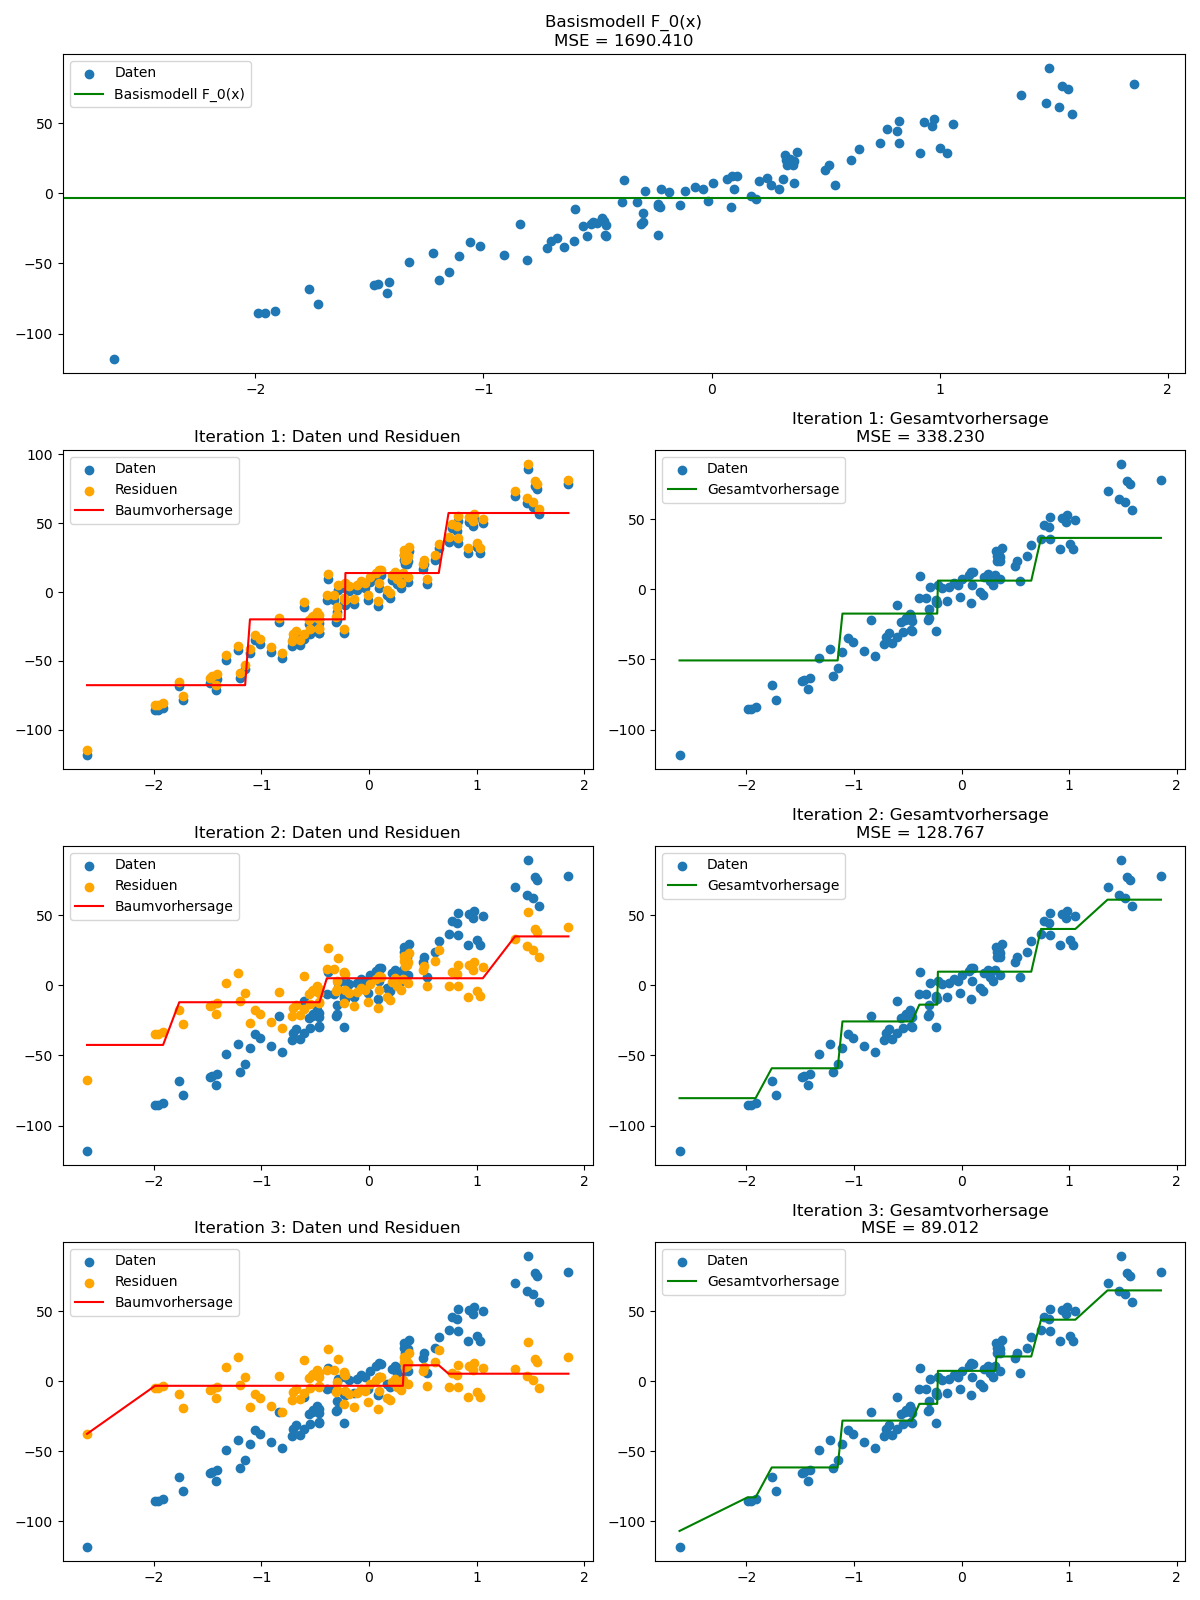
\includegraphics[width=0.8\textwidth]{Images/GBT_Example.png}
    \caption[Visualisierung des Gradient Boosting Trees Algorithmus]{Visualisierung des Gradient Boosting Trees Algorithmus.}
    \label{fig:gbt-example}
\end{figure}
\section{Vergleich von AdaBoost und Gradient Boosting}
In diesem Abschnitt werden die Unterschiede zwischen den Boosting-Algorithmen AdaBoost und Gradient Boosting (GBT) diskutiert. Wir betrachten ihre theoretischen Grundlagen, praktische Umsetzung, Vor- und Nachteile sowie typische Anwendungsfälle.

\subsection{Theoretische Grundlagen}
AdaBoost und GBT sind beides Ensemble-Lernmethoden, die auf dem Prinzip des Boosting basieren. AdaBoost konzentriert sich darauf, die Gewichte von Trainingsdaten anzupassen, um die Fehler der vorherigen Lerner zu korrigieren. Dies führt zu einer sequenziellen Anpassung, bei der jeder nachfolgende Lerner versucht, die Schwächen des Vorgängers zu verbessern. 
\newline
\newline
Im Gegensatz dazu arbeitet GBT mit Entscheidungsbäumen und konzentriert sich auf die Minimierung einer differenzierbaren Verlustfunktion, häufig unter Verwendung von Gradientenabstiegsverfahren. Dieser Ansatz ermöglicht es GBT, sowohl für Klassifikations- als auch für Regressionsprobleme effektiv zu sein.

\subsection{Praktische Umsetzung}
In der praktischen Anwendung wird AdaBoost häufig bei binären Klassifikationsproblemen eingesetzt, während GBT seine Stärken in komplexen Regressionsproblemen und multiklassen Klassifikationsaufgaben zeigt. AdaBoost ist in der Regel schneller in der Trainingsphase, da es einfacher in seiner Struktur ist. GBT hingegen, kann durch seine Flexibilität in der Anpassung von Entscheidungsbäumen und Verlustfunktionen komplexere Muster in den Daten erfassen.

\subsection{Vor- und Nachteile}
Ein wesentlicher Vorteil von AdaBoost liegt in seiner Einfachheit und Effizienz. Es ist leicht zu implementieren und bietet gute Ergebnisse bei einer Vielzahl von Problemen. Allerdings ist AdaBoost anfällig für Überanpassung, insbesondere bei Rauschen und Ausreißern in den Daten.
\newline
\newline
GBT hingegen ist flexibler und leistungsfähiger bei der Handhabung verschiedener Arten von Datenstrukturen und Verteilungen. Es kann jedoch rechenintensiver sein und erfordert eine sorgfältigere Abstimmung der Hyperparameter.

\subsection{Einsatzgebiete und Leistungsbewertung}
AdaBoost wird häufig in Anwendungen eingesetzt, bei denen die Geschwindigkeit der Modellerstellung kritisch ist und die Daten relativ frei von Ausreißern sind. GBT hingegen findet Anwendung in Szenarien, bei denen die Genauigkeit des Modells von höchster Bedeutung ist, wie beispielsweise in fortgeschrittenen Analytiken oder bei komplexen Regressionsproblemen.

\subsubsection{Datensatz `california housing'}
Um diese Unterschiede zu veranschaulichen habe ich mich für eine komplexe Regressiononsaufgabe, den bekannten Datensatz zu den Wohnungsdaten in Kalifornien, entschieden. Ziel bei diesem Datensatz ist es, den Hauspreis zu schätzen. Die Visualisierung, sowie die verwendeten Daten ist ein eigenes Beispiel und wurde mithilfe von SKLearn in python erstellt. Die genaue Implementierung ist auf meinem \textbf{\href{https://github.com/CodeLtDave/Boosting-Algorithms-ML-Seminararbeit/blob/main/python-env/VergleichAdaBoostGBT.ipynb}{GitHub}} zu finden.

\begin{table}[ht]
    \centering
    \caption{Beispieldaten aus dem Kalifornien Wohnungsdatensatz}
    \label{tab:housing_data}
    \resizebox{\textwidth}{!}{
    \begin{tabular}{rrrrrrrrr}
\toprule
MedInc & HouseAge & AveRooms & AveBedrms & Population & AveOccup & Latitude & Longitude & Hauspreis \\
\midrule
8.33 & 41.00 & 6.98 & 1.02 & 322.00 & 2.56 & 37.88 & -122.23 & 4.53 \\
8.30 & 21.00 & 6.24 & 0.97 & 2401.00 & 2.11 & 37.86 & -122.22 & 3.58 \\
7.26 & 52.00 & 8.29 & 1.07 & 496.00 & 2.80 & 37.85 & -122.24 & 3.52 \\
5.64 & 52.00 & 5.82 & 1.07 & 558.00 & 2.55 & 37.85 & -122.25 & 3.41 \\
3.85 & 52.00 & 6.28 & 1.08 & 565.00 & 2.18 & 37.85 & -122.25 & 3.42 \\
\bottomrule
\end{tabular}

    }
\end{table}
    

\begin{figure}[ht]
    \centering
    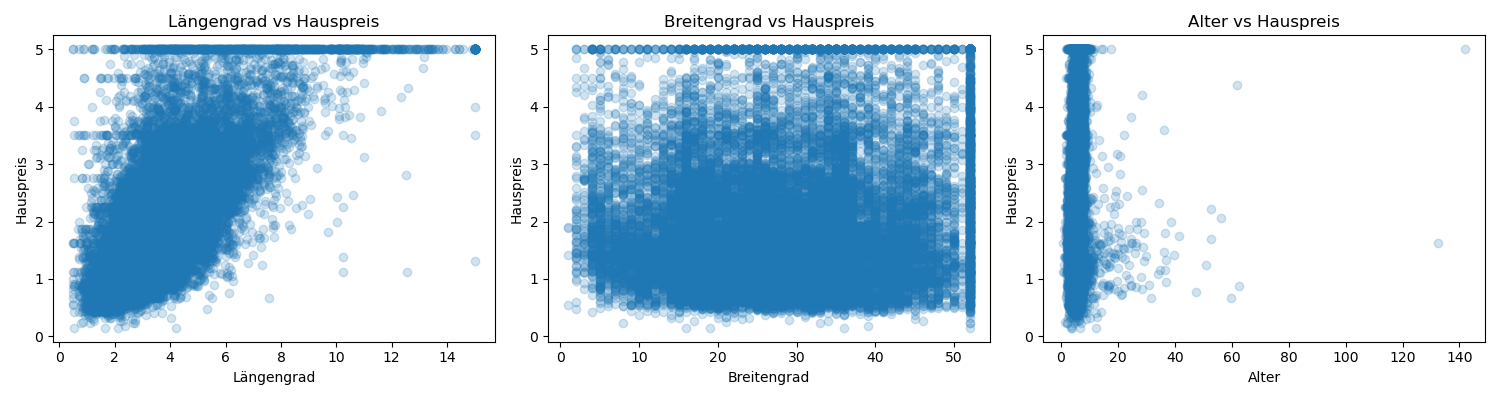
\includegraphics[width=\textwidth]{Images/housing_features.png}
    \caption{Visualisierung von Merkmalen des Kalifornien Wohnungsdatensatzes}
    \label{fig:housing_features}
\end{figure}

\subsubsection{Leistungsvergleich}
Abbildung \ref{fig:housing_performance} zeigt einen Vergleich der Leistung von AdaBoost und GBT auf `california housing' Datensatz. Es wird deutlich, dass GBT in Bezug auf den mittleren quadratischen Fehler (MSE) besser abschneidet, was seine Eignung für komplexe Regressionsprobleme unterstreicht. Allerdings ist AdaBoost deutlich schneller bei der Berechnung gewesen. Auf einem für AdaBoost besser geeigneten Datensatz wäre also GBT weniger effizient.

\begin{figure}[ht]
    \centering
    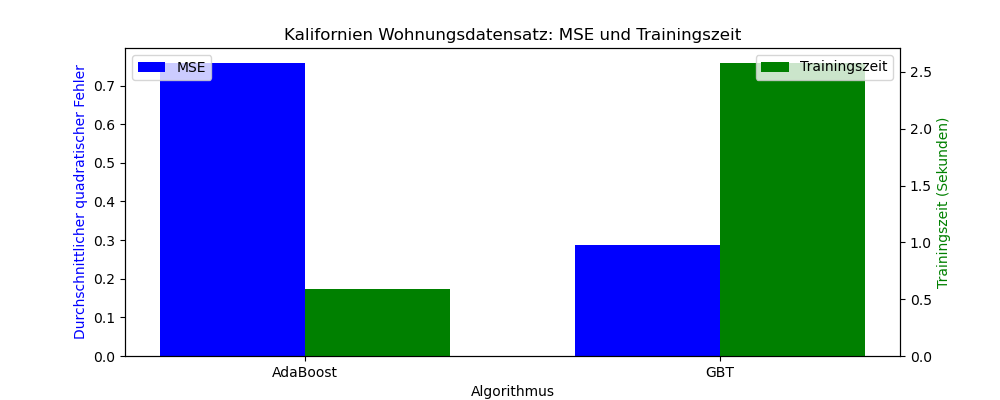
\includegraphics[width=0.8\textwidth]{Images/housing_performance.png}
    \caption{Leistungsvergleich von AdaBoost und GBT auf dem Kalifornien Wohnungsdatensatz}
    \label{fig:housing_performance}
\end{figure}

\section{Aktuelle Trends und Entwicklungen (2-3 Seiten)}
\subsection{Neueste Forschungsergebnisse}
\subsection{Zukünftige Potenziale von Boosting-Algorithmen}

\subsection{Toleranz gegen Overfitting}
!!! VERWEISEN

\subsection{Exponentieller Abstieg des Trainingfehlers}
!!! VERWEISEN


\section {Vergleich mit anderen ML-Modellen}

%%| GLOSSARY IMPORT |%%
\newglossaryentry{adaboost}{
  name=AdaBoost,
  description={Ein Machine Learning-Algorithmus, der auf dem Prinzip des Boosting basiert.}
}
\newglossaryentry{gradientboosting}{
  name=Gradient Boosting,
  description={Eine Methode des maschinellen Lernens, die für Regression und Klassifikation verwendet wird.}
}


%%%%%%%%%%%%%%%%%%%%%%%%%%%%%%%%%%%%%%%%%%%%%%%%%%%%%%%%%%%%%%%%%%%%%%%%%%%%%%%%%%%%%%%%%%%%%%%%%%%%%%%%%%%%%%%%%%%%%%%%%%%%%%%%%%%%%%%
%%| GLOSSARY |%%   
\newpage    
\printglossaries{}

%%%%%%%%%%%%%%%%%%%%%%%%%%%%%%%%%%%%%%%%%%%%%%%%%%%%%%%%%%%%%%%%%%%%%%%%%%%%%%%%%%%%%%%%%%%%%%%%%%%%%%%%%%%%%%%%%%%%%%%%%%%%%%%%%%%%%%%
%%| BIBLIOGRAPHY |%%                 
\newpage                                          
\printbibliography[heading=bibintoc, title={Literaturverzeichnis}]

%%| FIGURES AND TABLES LISTS |%%
\newpage
\listoffigures
\addcontentsline{toc}{section}{Abbildungsverzeichnis}
\newpage
\listoftables
\addcontentsline{toc}{section}{Tabellenverzeichnis}
\newpage
\listofalgorithms
\addcontentsline{toc}{section}{Algorithmenverzeichnis}

\end{document}
